\documentclass[10pt, conference, compsocconf, letterpaper]{IEEEtranv17}

\pagestyle{plain}

\usepackage{algorithm}
%\usepackage{times}
\usepackage{amsmath}
\usepackage{amsthm}
\usepackage{graphicx}
\usepackage{color}
\usepackage{amssymb}
\usepackage[noend]{distribalgo}
\usepackage[draft]{fixme}
\usepackage{soul}
% natbib and cite added by me, not part of the ieeetran template!
%\usepackage[numbers]{natbib}
%\usepackage{cite}

\newcommand{\ex}{$\mathcal{E}$}
\newcommand{\pp}{$\mathcal{P}$}
\newcommand{\ppm}{\mathcal{P}}
\newcommand{\cc}{$\mathcal{C}$}
\newcommand{\ccm}{\mathcal{C}}
\newcommand{\vv}{$\mathcal{V}$}
\newcommand{\vvm}{\mathcal{V}}
\newcommand{\rr}{$\mathcal{R}$}
\newcommand{\rrm}{\mathcal{R}}
\newcommand{\sst}{$\mathcal{S}$}
\newcommand{\ssm}{\mathcal{S}}
\newcommand{\ts}{\text{\textit{ts}}}
\newcommand{\sendersTo}{\text{\textit{sendersTo}}}
\newcommand{\readv}{\text{\textit{read}}}
\newcommand{\writev}{\text{\textit{write}}}
\newcommand{\comp}{\text{\textit{computation}}}
\newcommand{\send}{\text{\textit{send}}}
\newcommand{\recv}{\text{\textit{receive}}}

\begin{document}

%\title{Scalable State-Machine Replication}
%
%
%\author{
%    \IEEEauthorblockN{Carlos Eduardo Bezerra\IEEEauthorrefmark{1}\IEEEauthorrefmark{3}, Fernando Pedone\IEEEauthorrefmark{1}, Robbert van Renesse\IEEEauthorrefmark{2}}
%    \IEEEauthorblockA  {
%       \IEEEauthorrefmark{1}University of Lugano,
%       \IEEEauthorrefmark{2}Cornell University,
%       \IEEEauthorrefmark{3}Universidade Federal do Rio Grande do Sul
%    }
%}

\title {Scalable State-Machine Replication\\[-3.0ex]}
\author {
    \IEEEauthorblockN {
        Carlos Eduardo Bezerra\IEEEauthorrefmark{1}\IEEEauthorrefmark{3},
        Fernando Pedone\IEEEauthorrefmark{1},
        Robbert van Renesse\IEEEauthorrefmark{2}
    }
    \IEEEauthorblockA {\IEEEauthorrefmark{1}University of Lugano, Switzerland}
    \IEEEauthorblockA {\IEEEauthorrefmark{2}Cornell University, USA}
    \IEEEauthorblockA {\IEEEauthorrefmark{3}Universidade Federal do Rio Grande do Sul, Brazil}
    \\[-3.0ex]
}

%\title{Scalable State-Machine Replication\\[3.0ex] 
%  {\normalfont\normalsize
%    Carlos Eduardo Bezerra\IEEEauthorrefmark{1}\IEEEauthorrefmark{3}, Fernando Pedone\IEEEauthorrefmark{1}, Robbert van Renesse\IEEEauthorrefmark{2}
%  }\\[-4.5ex]}
%
%\author{
%    \IEEEauthorblockA  {
%        \IEEEauthorrefmark{1}University of Lugano\\
%        Switzerland\\
%    }
%    \and
%    \IEEEauthorblockA  {
%        \IEEEauthorrefmark{2}Cornell University\\
%        United States of America
%    }
%    \and
%    \IEEEauthorblockA  {
%        \IEEEauthorrefmark{3}Universidade Federal do Rio Grande do Sul\\
%        Brazil
%    }
%}

\maketitle




Sharding and replication are the mechanisms of choice of most scalable and fault-tolerant distributed systems.
The performance of a sharded system, however, heavily depends on the partitioning of the data: in order to scale, most commands must involve a single shard and load must be balanced across shards.
Estimating a good partitioning of the application state is challenging since it requires a priori information about the workload.
Moreover, even if such information is available, access patterns may change during system execution.
A good partitioning of the data for uniform access patterns may lead to poor performance under skewed access patterns.
The paper introduces DynaStar, a scalable and fault-tolerant system that supports dynamic state partitioning.
This means that DynaStar does not require a priori knowledge about the workload and can seamlessly adapt to workload variations.
The paper describes DynaStar design and implementation, and presents a detailed performance evaluation using two benchmarks, a social network based on real data and TPC-C.



%!TEX root =  ssmr_ieee.tex

\section{Introduction}
\label{sec:introduction}

Many current online services have stringent availability and performance requirements.
High availability entails tolerating component failures and is typically accomplished with replication.
For many online services, ``high performance" essentially means the ability to serve an arbitrarily large load, something that can be achieved if the service can scale throughput with the number of replicas.
% as the load increases (i.e., as more client requests are submitted by unit of time).
%
State machine replication (SMR)~\cite{Lam78, Sch90} is a well-known technique to provide fault tolerance without sacrificing strong consistency (i.e., linearizability).
%
%\ul{SMR consists of having replicas executing all clients requests in the same order. It usually requires each request execution to be deterministic, in which case the execution will lead to the same state in every replica.} 
SMR regulates how client commands are propagated to and executed by the replicas: every \mbox{non-faulty} replica must receive and execute every command in the same order. Moreover, command execution must be deterministic.
%
SMR provides configurable availability, by setting the number of replicas, but limited scalability: every replica added to the system must execute all requests; hence, throughput does not increase as replicas join the system.

Distributed systems usually rely on state partitioning to scale (e.g., \cite{facebookTAO, sciascia2012sdur}).
If requests can be served simultaneously by multiple partitions, then augmenting the number of partitions results in an overall increase in system throughput.
%, i.e., the system can scale throughput with the number of partitions.
However, exploiting state partitioning in SMR is challenging:
First, ensuring linearizability efficiently when state is partitioned is tricky.  
To see why, note that the system must be able to order multiple streams of commands simultaneously (e.g., one stream per partition) since totally ordering all commands cannot scale.
But with independent streams of ordered commands, how to handle commands that address multiple partitions?
%
Second, SMR hides from the service designer much of the complexity involved in replication; all the service designer must provide is a sequential implementation of each service command.
If state is partitioned, then some commands may need data from multiple partitions.
Should the service designer introduce additional logic in the implementation to handle such cases?
Should the service be limited to commands that access a single partition?

This paper presents Scalable State Machine Replication (S-SMR), an approach that achieves scalable throughput and strong consistency (i.e., linearizability) without constraining service commands or adding additional complexity to their implementation.
%
S-SMR partitions the service state and relies on an atomic multicast primitive to consistently order commands within and across partitions.
We show in the paper that simply ordering commands consistently across partitions is not enough to ensure strong consistency in partitioned state machine replication.
S-SMR implements \emph{execution atomicity}, a property that prevents command interleaves that violate strong consistency. 
%Together with atomic multicast, it ensures linearizability for S-SMR (a detailed description is given in Section~\ref{sec:scalablesmr}).
%
To assess the performance of S-SMR, we developed Eyrie, a Java library that allows developers to implement partitioned-state services transparently, abstracting partitioning details, and Volery, a service that implements Zookeeper's API~\cite{ZOO2010}. 
All communication between partitions is handled internally by Eyrie, including remote object transfers. 
%To evaluate both S-SMR and the library, we used Eyrie to implemented Volery, a service that provides some functionalities of Zookeeper~\cite{ZOO2010}. 
In the experiments we conducted with Volery, throughput scaled with the number of partitions, in some cases linearly.
%, reaching 8 times the throughput of a single-partition Volery deployment when using 8 partitions. 
In some deployments, Volery reached over 250 thousand commands per second, largely outperforming Zookeeper, which served 45 thousand commands per second under the same workload.


The paper makes the following contributions: 
(1)~It introduces S-SMR and discusses several performance optimizations, including caching techniques.
(2)~It details Eyrie, a library to simplify the design of services based on S-SMR. 
(3)~It describes Volery to demonstrate how Eyrie can be used to implement a service that provides Zookeeper's API.
(4)~It presents a detailed experimental evaluation of Volery and compares its performance to Zookeeper.

The remainder of this paper is organized as follows.
Section~\ref{sec:model} describes our system model.
Section~\ref{sec:smr} presents state-machine replication and the motivation for this work.
Section~\ref{sec:scalablesmr} introduces S-SMR; we explain the technique in detail and argue about its correctness.
Section~\ref{sec:implementation} details the implementation of Eyrie and Volery.
Section~\ref{sec:evaluation} reports on the performance of the Volery service.
Section~\ref{sec:related_work} surveys related work and
Section~\ref{sec:conclusion} concludes the paper.

\clearpage

%!TEX root =  ssmr_ieee.tex

\section{Model and definitions}
\label{sec:model}

%In this section, we detail the system model and recall the notions of state-machine replication and linearizability, our correctness criterion.
%
%\subsection{Processes and communication}

We consider a distributed system consisting of an unbounded set of client processes $\ccm = \{c_1, c_2, ...\}$ and a bounded set of server processes $\ssm = \{s_1, ..., s_n\}$. 
Set $\ssm$ is divided into $P$ disjoint groups of servers, $\ssm_1, ..., \ssm_P$.
Processes are either \emph{correct}, if they never fail, or \emph{faulty}, otherwise. 
In either case, processes do not experience arbitrary behavior (i.e., no Byzantine failures).
Processes communicate by message passing, using either one-to-one or one-to-many communication, as defined next.
The system is asynchronous: there is no bound on message delay or on relative process speed.

One-to-one communication uses primitives $send(p,m)$ and $receive(m)$, where $m$ is a message and $p$ is the process $m$ is addressed to. 
If sender and receiver are correct, then every message sent is eventually received. 
%
One-to-many communication relies on atomic multicast, defined by the primitives \emph{multicast}$(\gamma, m)$ and \emph{deliver}$(m)$, where $\gamma$ is a set of server groups.
%where $g$ is the group message $m$ is addressed to, 
%
Let relation $\prec$ be defined such that $m \prec m'$ iff there is a server that delivers $m$ before $m'$.
Atomic multicast ensures that 
(i)~if a server delivers $m$, then all correct servers in $\gamma$ deliver $m$ \emph{(agreement)};
(ii)~if a correct process multicasts $m$ to groups in $\gamma$, then all correct servers in every group in $\gamma$ deliver $m$ \emph{(validity)}; and
(iii)~relation $\prec$ is acyclic \emph{(order)}.\footnote{Solving atomic multicast requires additional assumptions~\cite{CT96,FLP85}. In the following, we simply assume the existence of an atomic multicast oracle.}
%(ii)~if servers $s$ and $r$ deliver messages $m$ and $m'$, then they deliver them in the same order \emph{(order)}.
The order property implies that if $s$ and $r$ deliver messages $m$ and $m'$, then they deliver them in the same order. 
Atomic broadcast is a special case of atomic multicast in which there is a single group with all servers.



%!TEX root =  ssmr_ieee.tex

\section{Background and motivation}
%\section{State-machine replication}
\label{sec:smr}

State-machine replication is a fundamental approach to implementing a fault-tolerant service by replicating servers and coordinating the execution of client commands against server replicas~\cite{Lam78, Sch90}. 
The service is defined by a state machine, which consists of a set of \emph{state variables} $\vvm = \{v_1, ..., v_m\}$ 
%that encode the service's state 
and a set of \emph{commands} that may read and modify state variables, and produce a response for the command.
Each command is implemented by a deterministic program.
% whose execution is atomic with respect to other commands.
%The set of variables read by $C$ and the set of variables updated by $C$ are denoted, respectively, by $readset(C)$ and $writeset(C)$.
%The set of all variables read and updated by $C$ is denoted by $var(C)$. 
State-machine replication can be implemented with atomic broadcast: commands are atomically broadcast to all servers, and all correct servers deliver and execute the same sequence of commands.

We are interested in implementations of state-machine replication that ensure linearizability.
%
Linearizability is defined with respect to a sequential specification.
The \emph{sequential specification} of a service consists of a set of commands and a set of \emph{legal sequences of commands}, which define the behavior of the service when it is accessed sequentially.
In a legal sequence of commands, every response to the invocation of a command immediately follows its invocation, with no other invocation or response in between them.
For example, a sequence of operations for a read-write variable $v$ is legal if every read command returns the value of the most recent write command that precedes the read, if there is one, or the initial value otherwise.
An execution \ex\ is linearizable if there is some permutation of the commands executed in \ex\ that respects (i)~the service's sequential specification and (ii)~the real-time precedence of commands.
Command $C_1$ precedes command $C_2$ if the response of $C_1$ occurs before the invocation of $C_2$.

%The precise way in which the technique is implemented
%depends on the targeted consistency criterion, which in this paper we assume to be \emph{linearizability}. Once we prove that S-SMR provides such level of consistency, performance-optimized variations of S-SMR can be achieved later on by relaxing such consistency requirement. We can define linearizability intuitively: an execution in a replicated system is linearizable if the application program that uses such system gets the same behavior as with a single site, unreplicated system; hence, writing the application logic is no different to conventional programming~\cite{replication2010pedone}.

%To define linearizability more formally, we need the notion of \emph{sequential specification} for the variables, which determines whether a sequence of commands (and their matching responses) is legal, given a set of variables \mbox{$\vvm = \{v_1, ..., v_m\}$} stored in the servers. For example, the sequential specification for read-write variables is: given a sequence $\sigma$ of commands, the response given to any command $x$ that reads some variable $v$ must be coherent with the most recent command that writes $v$ and precedes $x$ in $\sigma$. Also, we need the notion of \emph{real-time precedence}, denoted by $<_{RT}$. We say that commands $x$ and $y$ are such that $x <_{RT} y$ if the response to command $x$ is received before command $y$ is issued, in real-time. Finally, execution \ex\ is linearizable if there is some permutation $\pi$ of the commands executed in \ex\, such that (i)~the sequential specification of every variable is respected in $\pi$ and (ii)~if $x <_{RT} y$, then $x$ precedes $y$ in $\pi$~\cite{Attiya04}.

%The execution in Fig.~\ref{fig:linvsnonlin} (top) is not linearizable because the reordering of commands that form a legal sequence (i.e., $C_1$, $C_3$, $C_2$) does not respect the real-time precedence of commands (i.e., it violates the real-time ordering of $C_2$ and $C_3$).
%%: we can see that $C_1 <_{RT} C_2 <_{RT} C_3$, but a permutation that respected such real-time precedence would not be legal. 
%In Fig.~\ref{fig:linvsnonlin} (bottom), however, there is no real-time precedence between $C_2$ and $C_3$, because $C_3$ was issued by client $b$ before client $a$ received the reply for $C_2$. For this reason, the execution is linearizable.
%
%\begin{figure}[ht]
%  \begin{center}
%    \begin{tabular}{c}
%      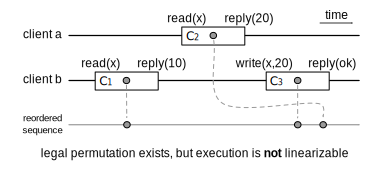
\includegraphics[width=0.9\columnwidth]{figures/nonlinearizable} \\
%      \\
%      \includegraphics[width=0.9\columnwidth]{figures/linearizable} \\
%    \end{tabular}
%    \caption{Linearizable vs. non-linearizable executions.}
%    \label{fig:linvsnonlin}
%  \end{center}
%% \vspace{-4mm}
%\end{figure}


%State-machine replication implements linearizability by regulating how client commands are propagated to and executed by the replicas: 
%(i)~every nonfaulty replica must receive every command;  and
%(ii)~replicas must agree on the order of received and executed commands.
%Since each command is implemented by a deterministic program, each replica will produce the same state changes and response upon executing the same sequence of commands.
%State-machine replication can be implemented with atomic broadcast: commands are atomically broadcast to all servers, and all correct servers deliver and execute the same sequence of commands.
%%Since execution is deterministic, every server reaches the same state and produces the same response after executing a  command.

%\subsection{On the (lack of) scalability of SMR}

In classical state-machine replication, throughput does not scale with the number of replicas: each command must be ordered among replicas and executed and replied by every (non-faulty) replica.
Some simple optimizations to the traditional scheme can provide improved performance but not scalability.
For example, although update commands must be ordered and executed by every replica, only one replica can respond to the client, saving resources at the other replicas.
Commands that only read the state must be ordered with respect to other commands, but can be executed by a single replica, the replica that will respond to the client.

%A simple analysis shows that these schemes do not scale with the number of servers.
%Assume a replica needs $\delta_o$ time units to order a command, $\delta_e$ time units to execute the command, and $\delta_r$ time units to respond to the client---for simplicity, we consider $\delta_o$ to be constant with the number of servers.
%%~\cite{Marandi10}.
%In this model, traditional state-machine replication has throughput of $1/(\delta_o+\delta_e+\delta_r)$.
%The optimizations for update and read-only commands improve throughput to $N/(\delta_o+\delta_e+\delta_r/N)$ and $N/(\delta_o+(\delta_e+\delta_r)/N)$, respectively, where $N$ is the number of replicas.
%A scalable system would have throughput that grows proportionally with the number of servers.
%Figure~\ref{fig:scale} compares the behavior of traditional state-machine replication and the update and read-only optimizations with a truly scalable implementation. In the figure, we assume $\delta_o=\delta_e=\delta_r$; different values of $\delta$ would not change the asymptotic behavior of the techniques.
%
%
%\begin{figure}[ht]
%  \begin{center}
%      \includegraphics[width=0.9\columnwidth]{graphs/smr-scal/scale.pdf} 
%    \caption{Scalability of SMR implementations.}
%        \label{fig:scale}
%  \end{center}
%\end{figure}


%Such traditional implementations of SMR, however, has limited scalability. Adding servers to the system may not increase its throughput, and is likely, instead, to create a larger overhead on the group-communication component of the system, responsible for implementing atomic multicast. Note that servers can divide the execution of read-only commands (only one server has to execute, since no state is changed) and the sending of replies to write commands (although the state must change in all servers, one reply is enough). In the best case, i.e., in a workload dominated by read-only commands, this would approximate a linear increase of throughput, relatively to the number of servers. However, the group communication component of the system would have to increase its capacity as well, in order to avoid becoming a bottleneck, but its cost, in number of internal messages, would grow linearly (at least) to the number of processes in such component,\footnote{To the best of our knowledge, Ring-Paxos~\cite{Marandi10} requires the lowest number of messages for a consensus algorithm, which is $O(a)$, where $a$ is the number of acceptors.} eventually weighing out the linear (at best) throughput gain. In any case, even with a read-only workload, every server would have to deliver every single command, which alone would prevent the system from scaling.

This is a fundamental limitation: while some optimizations may increase throughput by adding servers, the improvements are limited since fundamentally, the technique does not scale.
In the next section, we describe an extension to SMR that under certain workloads allows performance to grow proportionally to the number of replicas.


%State-machine replication can be implemented with atomic multicast: if all servers belong to the same group and all commands are atomically multicast to such group, then all correct servers deliver and execute the same sequence of commands, i.e., they execute the commands in the same order. Moreover, if all servers have each a full copy of the application state, they all start at the same initial state, and command execution is deterministic, then every server reaches the same state after executing a given command and, thus, no two servers give different responses to the same command.



%\clearpage

%!TEX root =  ssmr_ieee.tex
\section{Scalable State-Machine Replication}
\label{sec:scalablesmr}

In this section, we introduce S-SMR, discuss performance optimizations, and argue about S-SMR's correctness.
%In this section, we introduce Scalable State-Machine Replication (S-SMR), describing its general idea (Section~\ref{sec:generalidea}) and detail its algorithm (Section~\ref{sec:detailalg}), discuss performance optimisations (Section~\ref{sec:optm}), and argue about S-SMR's correctness (Section~\ref{sec:correctness}).


%\subsection{Baseline approach}
\subsection{General idea}
\label{sec:generalidea}

S-SMR divides the application state $\vvm$ (i.e., state variables) into $P$ partitions $\ppm_1, ..., \ppm_P$, where for each $\ppm_i$, $\ppm_i \subseteq \vvm$. 
Moreover, we require each variable $v$ in $\vvm$ to be assigned to at least one partition and define $part(v)$ as the partitions that hold $v$. 
Each partition $\ppm_i$ is replicated by servers in group $\ssm_i$.
For brevity, we say that server $s$ belongs to $\ppm_i$ with the meaning that $s \in \ssm_i$, and say that client $c$ multicasts command $C$ to partition $\ppm_i$ meaning that $c$ multicasts $C$ to group $\ssm_i$.
% We also say that $\ppm_i$ does something meaning that servers in $\ssm_i$.
%We also often mention $\ppm_i$ meaning servers in $\ssm_i$.

To execute command $C$, the client multicasts $C$ to all partitions that hold a variable read or updated by $C$.
Consequently, the client must be able to determine the partitions accessed by $C$, denoted by $part(C)$.
Note that this assumption does not imply that the client must know all variables accessed by $C$, but it must know the partitions these variables belong to.
If the client cannot accurately estimate which partitions are accessed by $C$, it must determine a superset of these partitions, in the worst case assuming all partitions.
For performance, however, clients must strive to provide a close approximation to the command's actually accessed partitions. We assume the existence of an oracle that tells the client which partitions should receive each command.

Upon delivering command $C$, if server $s$ does not contain all variables read by $C$, $s$ must communicate with servers in other partitions to execute $C$. 
%
%can execute $C$ without and send the response to the client that issued $C$.
%%
%If $s$ stores only some of the variables accessed by $C$, $s$ must communicate with servers in other partitions to execute $C$. 
Essentially, $s$ must retrieve every variable $v$ read in $C$ from a server that stores $v$ (i.e., a server in a partition in $part(v)$).
Moreover, $s$ must retrieve a value of $v$ that is consistent with the order in which $C$ is executed, as we explain next.
Operations that do not involve reading a variable from a remote partition are executed locally.
%Server $s$ executes write operations that modify variables it stores and discards the other write operations.

%In more detail, assume that command $C$ is formed by a sequence of operations $op(C)$.
%Let $read(v)$ be an operation that reads the value of a state variable $v$ and $write(v, val)$ an operation that updates $v$ with value $val$.
%Any other operation may depend only on the state values read and the command's input.
%In the following, we assume that all read operations in a command precede the write operations.
%; we revisit this assumption in Section~\ref{sec:optm}.
%
%Server $s$ in partition $\ppm_i$ executes the $k$-th operation in $C$, $op(C)[k]$, as follows.

In more detail, let $op$ be an operation in the execution of command $C$.
We distinguish between three operation types: $read(v)$, an operation that reads the value of a state variable $v$, $write(v, val)$, an operation that updates $v$ with value $val$,
%and an operation that is neither a read nor a write.
and an operation that performs a deterministic computation.

Server $s$ in partition $\ppm_i$ executes $op$ as follows.

\begin{itemize}

\item[i)] \underline{$op$ is a $read(v)$ operation.} \\
If $\ppm_i \in part(v)$, then $s$ retrieves the value of $v$ and sends it to every partition $\ppm_j$ that delivers $C$ and does not hold $v$. If $\ppm_i \not\in part(v)$, then $s$ waits for $v$ to be received from a server in a partition in $part(v)$.

\item[ii)] \underline{$op$ is a $write(v,val)$ operation.} \\
If $\ppm_i \in part(v)$, $s$ updates the value of $v$ with $val$; if $\ppm_i \not\in part(v)$, $s$ executes $op$, creating a local copy of $v$, which will be up-to-date at least until the end of $C$'s execution.

\item[iii)] \underline{$op$ is a computation operation.}\\
In this case, $s$ executes $op$.

\end{itemize}

As we now show, the procedure above does not ensure linearizability.
Consider the execution depicted in Figure~\ref{fig:mcastnonlinssmr}~(a), where state variables $x$ and $y$ have initial value of $10$. 
Command $C_x$ reads the value of $x$, $C_y$ reads the value of $y$, and $C_{xy}$ sets $x$ and $y$ to value 20.
Consequently, $C_x$ is multicast to partition $\ppm_x$, $C_y$ is multicast to $\ppm_y$, and $C_{xy}$ is multicast to both $\ppm_x$ and $\ppm_y$. 
Servers in $\ppm_y$ deliver $C_y$ and then $C_{xy}$, while servers in $\ppm_x$ deliver $C_{xy}$ and then $C_x$, which is consistent with atomic order. 
In this execution, the only possible legal permutation for the commands is $C_y$, $C_{xy}$, and $C_x$, which violates the real-time precedence of the commands, since $C_x$ precedes $C_y$ in real-time.

%\begin{figure}[ht]
%  \begin{center}
%    \begin{tabular}{c}
%      \includegraphics[width=0.9\columnwidth]{figures/mcastnonlinssmr} \\
%    \end{tabular}
%    \caption{Atomic multicast and S-SMR.}
%    \label{fig:mcastnonlinssmr}
%  \end{center}
%% \vspace{-4mm}
%\end{figure}
%
\begin{figure*}
\begin{minipage}[b]{1.0\linewidth} % A minipage that covers the whole width of the page
\centering
      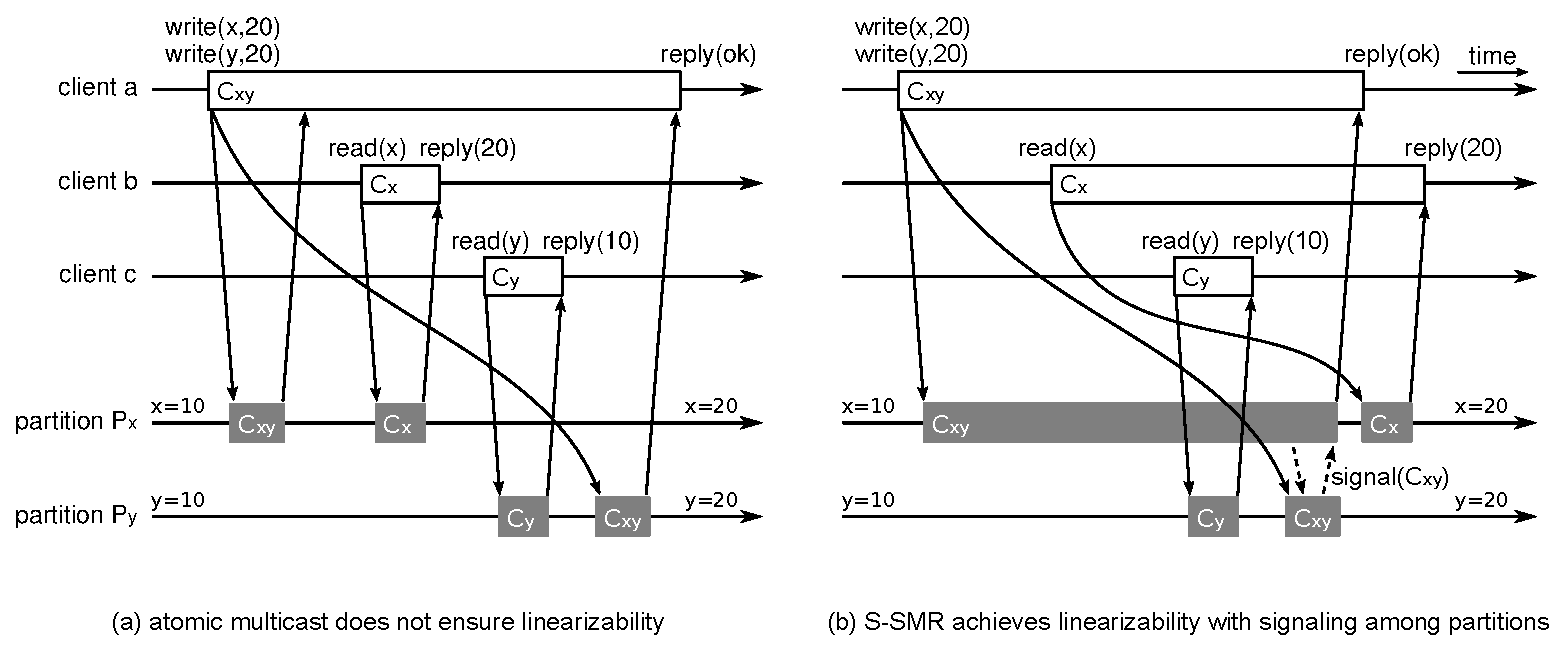
\includegraphics[width=0.85\linewidth]{figures/mcastssmr_nonlin_linsignal_v3}
\end{minipage}
%\begin{minipage}[b]{0.5\linewidth} % A minipage that covers half the page
%\centering
%      \includegraphics[width=0.9\columnwidth]{figures/mcastnonlinssmr}
%\end{minipage}
%\begin{minipage}[b]{0.5\linewidth}
%\centering
%      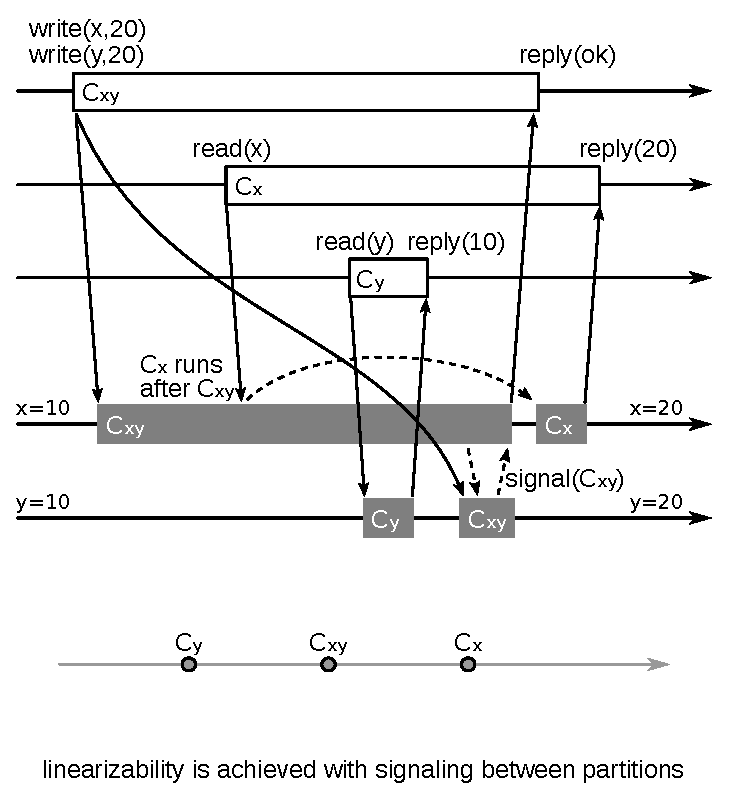
\includegraphics[width=0.9\columnwidth]{figures/mcastlinssmr_signal}
%\end{minipage}
\caption{Atomic multicast and S-SMR. (To simplify the figure, we show a single replica per partition.)}
\label{fig:mcastnonlinssmr}
\end{figure*}

Intuitively, the problem with the execution in Figure~\ref{fig:mcastnonlinssmr}~(a) is that commands $C_x$ and $C_y$ execute ``in between" the execution of $C_{xy}$ at partitions $\ppm_x$ and $\ppm_y$.
In S-SMR, we avoid such cases by ensuring that the execution of every command is atomic.
%
Command $C$ is \emph{execution atomic} if, for each server $s$ that executes $C$, there exists at least one server $r$ in every other partition in $part(C)$ such that the execution of $C$ at $s$ finishes after $r$ delivers $C$.
%
More precisely, let $delivery(C,s)$ and $end(C,s)$ be, respectively, the time when $s$ delivers command $C$ and the time when $s$ completes $C$'s execution.
Execution atomicity ensures that, for every server $s$ in partition \pp\ that executes $C$, there is a server $r$ in every $\ppm' \in part(C)$ such that $delivery(C,r) < end(C,s)$.
Intuitively, this condition guarantees that the execution of $C$ at $\ppm$ and $\ppm'$ overlap in time.

%Back in Fig.~\ref{fig:mcastnonlinssmr}, each black box represents the execution of a subcommand by servers in the partition: it starts when the first server in the partition begins executing the subcommand and ends when there is no more server executing the subcommand in that partition. We can see that $C_{xy}$ is not execution atomic: there is no time $t$ when some servers $s_x$ in $P_x$ and $s_y$ in $P_y$ are executing it. If it were the case, this example would be impossible to build, since $finish(C_y,s_y) < start(C_{xy}, s_y) < t < finish(C_{xy}, s_x) < start(C_x, s_x)$, which would contradict the fact that $C_x$ precedes $C_y$ in real-time.

Replicas can ensure execution atomicity by coordinating the execution of commands.
After delivering command $C$, servers in each partition send a $signal(C)$ message to servers in the other partitions in $part(C)$.
Before finishing the execution of $C$, each server must receive a $signal(C)$ message from at least one server in every other partition that executes $C$. 
%To minimize the waiting time to complete the execution of commands, servers may send such signal as soon as they deliver the command.
Moreover, if server $s$ in partition $\ppm$ receives the value of a variable from server $r$ in another partition $\ppm'$, as part of the execution of $C$, then $s$ does not need to receive a $signal(C)$ message from servers in $\ppm'$. This way, to tolerate $f$ failures, each partition requires $f+1$ servers; if all servers in a partition fail, service progress is not guaranteed.

Figure \ref{fig:mcastnonlinssmr}~(b) shows an execution of S-SMR. 
In the example, servers in $P_x$ wait for a signal from $P_y$, therefore delaying $C_{xy}$'s execution in $P_x$ and moving the execution of $C_x$ ahead in time. 
Note that the outcome of each command execution is the same as in case (a), but the executions of $C_x$, $C_y$ and $C_{xy}$, as seen by clients, now overlap in time with one another. 
Hence, there is no real-time precedence among them.

\subsection{Detailed algorithm}
\label{sec:detailalg}


\begin{algorithm}
\small
%\footnotesize
\begin{distribalgo}[1]
%\STATE \textbf{Algorithm 1:\\} Scalable State-Machine Replication (S-SMR)
\vspace{1mm}

\INDENT{\emph{Initialization:}}
    \STATE $\forall C \in \mathcal{K} : rcvd\_signals(C) \leftarrow \emptyset$
    \STATE $\forall C \in \mathcal{K} : rcvd\_variables(C) \leftarrow \emptyset$
\ENDINDENT

\vspace{1.5mm}
%\vspace{2.0mm}
\INDENT{\emph{Command $C$ is submitted by a client as follows:}}
    \STATE $dests \leftarrow oracle(C)$ \label{algline:oracle} 
%    \COMMENT{$oracle(C)$ returns a superset of $part(C)$}
	\STATE multicast$(dests, C)$ \label{algline:climcast}
	\STATE wait for response from one server
\ENDINDENT

\vspace{1.5mm}
%\vspace{2.0mm}
\INDENT{\emph{Command $C$ is executed by a server in partition \pp\ as follows:}}
	\INDENT{\textbf{upon} deliver$(C)$}
	    \STATE $others \leftarrow dests \setminus \{\ppm\}$ \label{algline:others}
	    \STATE multicast$(others, signal(C))$ \label{algline:mcastsignals}
		\FOR{each operation $op$ in $C$}
			\IF{$op$ is $read(v)$}
			    \IF{$v \in \ppm$}
			        \STATE multicast$(others, \{v,C.id\})$ \label{algline:multicastv}
			    \ELSE
			        \STATE \textbf{wait until} $v \in rcvd\_variables(C)$ \label{algline:waitvariable}
			        \STATE update $v$ with the value in $rcvd\_variables(C)$
			    \ENDIF
			\ENDIF
			\STATE execute $op$ \label{algline:executeopck}
		\ENDFOR
		\STATE \textbf{wait until} $rcvd\_signals(C) = others$ \label{algline:waitsignals}
		\STATE send reply to client \label{algline:sendreply}
	\ENDINDENT
	
	\vspace{2.0mm}
	\INDENT{\textbf{upon} deliver$(signal(C))$ from partition $\ppm'$}
	    \STATE $rcvd\_signals(C) \leftarrow rcvd\_signals(C) \cup \{\ppm'\}$
	\ENDINDENT

	\vspace{2.0mm}
	\INDENT{\textbf{upon} deliver$(\{v, C.id\})$}
	    \STATE $rcvd\_variables(C) \leftarrow rcvd\_variables(C) \cup \{v\}$
	\ENDINDENT
			
\ENDINDENT

\vspace{1.5mm}
%\vspace{2mm}

\textbf{Algorithm variables:}

\vspace{1mm}

$\mathcal{K}$: the set of all possible commands

\vspace{1mm}

$C.id$: unique identifier of command $C$

\vspace{1mm}

$oracle(C)$: function that returns a superset of $part(C)$

\vspace{1mm}

$dests$: set of partitions to which $C$ is multicast

\vspace{1mm}

$others$: set of partitions waiting for signals and variables from \pp; also, \pp\ waits for signals from all such partitions

\vspace{1mm}

$signal(C)$: a synchronization message that allows S-SMR to ensure $C$ to be execution atomic

\vspace{1mm}

$rcvd\_signals(C)$: a set containing all partitions that already signaled \pp\ regarding the execution of $C$

\vspace{1mm}

$rcvd\_variables(C)$: a set containing all variables that must be received from other partitions in order to execute $C$

\caption{Scalable State-Machine Replication (S-SMR)}
\label{alg:ssmr}
\end{distribalgo}
\end{algorithm}

In Algorithm \ref{alg:ssmr}, we show the basic operation of S-SMR. 
To submit a command $C$, the client queries an oracle to get set $dests$~(line \ref{algline:oracle}), which is a superset of $part(C)$ used by the client as destination set for $C$~(line \ref{algline:climcast}).

Upon delivering $C$, server $s$ in partition \pp\ multicasts $signal(C)$ to $others$, which is the set containing all other partitions involved in $C$ (lines \ref{algline:others} and \ref{algline:mcastsignals}). 
%The purpose of $signal(C)$ is to let servers in other partitions know that there is a server in \pp\ that started executing $C$. 
It might happen that $s$ receives signals concerning $C$ from other partitions even before $s$ started executing $C$. For this reason, $s$ must buffer signals and check if there are signals buffered already when starting the execution of $C$. For the sake of simplicity, Algorithm \ref{alg:ssmr} simply initializes such buffers as $\emptyset$ for all possible commands. In practice, buffers for $C$ are created when the first message concerning $C$ is delivered.

After multicasting signals, server $s$ proceeds to the execution of $C$, which is a sequence of operations that might read or write variables in \vv. The main concern is with operations that read variables, as they may determine the outcome of the command execution. All other operations can be executed locally at $s$. If the operation reads variable $v$ and $v$ belongs to \pp, $s$'s partition, then $s$ multicasts the value of $v$ to the other partitions that delivered $C$ (line \ref{algline:multicastv}). The command identifier $C.id$ is sent along with $v$ to make sure that the other partitions will use the appropriate value of $v$ during $C$'s execution. If $v$ belongs to some other partition $\ppm'$, $s$ waits until an up-to-date value of $v$ has been delivered (line \ref{algline:waitvariable}). Every other operation is executed with no interaction with other partitions (line \ref{algline:executeopck}).

After executing all operations of $C$, $s$ waits until a signal from every other partition has been received (line \ref{algline:waitsignals}) and, only then, sends the reply back to the client (line \ref{algline:sendreply}). This ensures that $C$ will be execution atomic.



\subsection{Performance optimizations}
\label{sec:optm}

Algorithm \ref{alg:ssmr} can be optimized in many ways. 
In this section, we briefly mention some of these optimizations and then detail caching.
\begin{itemize}
\item Server $s$ does not need to wait for the execution of command $C$ to reach a $read(v)$ operation to only then multicast $v$ to the other partitions in $part(C)$. If $s$ knows that $v$ will be read by $C$, $s$ can send $v$'s value to the other partitions as soon as $s$ starts executing $C$.
\item The exchange of objects between partitions serves the purpose of signaling. Therefore, if server $s$ sends variable $v$'s value to server $r$ in another partition, $r$ does not need to receive a signal message from $s$'s partition.
\item It is not necessary to exchange each variable more than once per command since any change during the execution of the command will be deterministic and thus any changes to the variable can be applied to the cached value.
\item Even though all replicas in all partitions in $part(C)$ execute $C$, a reply from a replica in a single partition suffices for the client to finish the command.
\end{itemize}

%Caching is a more elaborate optimization. 
Server $s$ in partition \pp\ can cache variables that belong to other partitions. 
There are different ways for $s$ to maintain cached variables; here we define two techniques: conservative caching and speculative caching. 
In both cases, the basic operation is the following: 
When $s$ executes a command that reads variable $x$ from some other partition $\ppm{}_x$, after retrieving the value of $x$ from a server in $\ppm{}_x$, $s$ stores $x$'s value in its cache and uses the cached value in future read operations.
If a command writes $x$, $s$ updates (or creates) $x$'s local value. 
Server $s$ will have a valid cache of $x$ until (i)~$s$ discards the entry due to memory constraints, or (ii)~some command not multicast to \pp\ changes the value of $x$. 
Since servers in $\ppm_x$ deliver all commands that access $x$, these servers know when any possible cached value of $x$ is stale.
How servers use cached entries distinguishes conservative from speculative caching.
%; what it does not know, however, is whether \pp\ has discarded $x$'s cache. 


Servers in $\ppm_x$ can determine which of its variables have a stale value cached in other partitions. This can be done by checking if there was any command that updated a variable $x$ in $\ppm_x$, where such command was not multicast to some other partition $\ppm$ that had a cache of $x$. Say servers in $\ppm_x$ deliver command $C$, which reads $x$, and say the last command that updated the value of $x$ was $C_w$. Since $x \in \ppm_x$, servers in $\ppm_x$ delivered $C_w$. One way for servers in $\ppm_x$ to determine which partitions need to update their cache of $x$ is by checking which destinations of $C$ did not receive $C_w$. This can be further optimized: even if servers in $\ppm$ did not deliver $C_w$, but delivered some other command $C_r$ that reads $x$ and $C_r$ was ordered by multicast after $C_w$, then $\ppm$ already received an up-to-date value of $x$ (sent by servers in $\ppm_x$ during the execution of $C_r$). If servers in $\ppm$ discarded the cache of $x$ (e.g., due to limited memory), they will have to send a request for its value.


\emph{Conservative caching}: Once $s$ has a cached value of $x$, before it executes a $read(x)$ operation, it waits for a cache-validation message from a server in $\ppm_x$. The cache validation message contains a set of pairs $(var, val)$, where $var$ is a state variable that belongs to $\ppm_x$ and whose cache in $\ppm$ needs to be validated. 
If servers in $\ppm_x$ determined that the cache is stale, $val$ contains the new value of $var$; otherwise, $\perp$, telling $s$ that its cached value is up to date.
If $s$ discarded its cached copy, it sends a request for $x$ to $\ppm_x$.
If it is possible to determine which variables are accessed by $C$ before $C$'s execution, all such messages can be sent upon delivery of the command, reducing waiting time; messages concerning variables that could not be determined a-priori are sent later, during the execution of $C$, as variables are determined.

\emph{Speculative caching}: It is possible to reduce execution time by speculatively assuming that cached values are up-to-date. 
Speculative caching requires servers to be able to rollback the execution of commands, in case the speculative assumption fails to hold. 
Many applications allow rolling back a command, such as databases, as long as no reply has been sent to the client for the command yet. 
The difference between speculative caching and conservative caching is that in the former servers that keep cached values do not wait for a cache-validation message before reading a cached entry; instead, a $read(x)$ operation returns the cached value immediately. 
If after reading some variable $x$ from the cache, during the execution of command $C$, server $s$ receives a message from a server in $\ppm_x$ that invalidates the cached value, $s$ rolls back the execution to some point before the $read(x)$ operation and resumes the command execution, now with the up-to-date value of $x$. 
%This may happen for every variable read by $C$, so $s$ might rollback the execution of $C$ several times until getting it right. 
%To ensure that a correct execution will be done eventually, 
Server $s$ can only reply to the client that issued $C$ after every variable read from the cache has been validated.

%Both caching algorithms depend on the following condition: each partition $\ppm_x$ keeps track of what was the last command $C$ executed by each partition $\ppm$, for each variable $x$ in $\ppm_x$, such that $C$ reads or writes $x$.\fixme{This part is too complicated.}
%Such values are kept by $\ppm_x$ in a table where each entry is $\langle \ppm, x, k \rangle$, where $k$ identifies the last command executed by $\ppm$ that accesses $x$. The initial value of $k$ is $0$ for every partition and every variable. Whenever a command $C$ that accesses $x$ is delivered by $\ppm_x$, it increments the command counter $k$ in $\langle \ppm, x, k \rangle$, for every partition $\ppm$ that delivers $C$. Upon delivery of any command $C'$ that also accesses $x$, $\ppm_x$ checks whether there is any partition $\ppm'$ that $C'$ was multicast to, where the cache of $x$ read by $C'$ will be stale, that is, entries $\langle \ppm_x, x, k \rangle$ and $\langle \ppm', x, k' \rangle$ are such that $k' < k$. Then, $P_x$ sends the cache-validation message(s) to $\ppm'$ accordingly.

\subsection{Correctness}
\label{sec:correctness}

In this proof, we denote the order given by atomic multicast with ``$\prec$''. Given any two messages $m_1$ and $m_2$, ``$m_1 \prec m_2$'' means that both messages are delivered by the same group and $m_1$ is delivered before $m_2$, or there is some message $m'$ such that $m_1 \prec m'$ and $m' \prec m_2$, which can be written as \mbox{$m_1 \prec m' \prec m_2$}.

We argue that, if every command in execution \ex\ of \mbox{S-SMR} is execution atomic, then \ex\ is linearizable. Suppose, by means of contradiction, that there exist two commands $x$ and $y$, where $x$ finishes before $y$ starts, but $y \prec x$ in the execution. There are two possibilities for this: (i) $x$ and $y$ access some variable in common $v$, or (ii) $x$ and $y$ access no variable in common.

In case (i), at least one partition $P_v$ (which contains $v$) delivers both $x$ and $y$. As $x$ finishes before $y$ starts, then $P_v$ delivers $x$, then $y$. From the properties of atomic multicast, and since each partition is mapped to a multicast group, no partition delivers $y$, then $x$. Moreover, atomic multicast ensures acyclic order, so there are no commands $z_1, ..., z_n$ such that their atomic order is $y \prec z_1 \prec \cdots \prec z_n \prec x$. So, we reached a contradiction in this case.

In case (ii), if there were no other command in \ex, then the execution of $x$ and $y$ could be done in any order, which would contradict the supposition that $y \prec x$. Therefore, there are commands $z_0, ..., z_n$ such that their atomic order is $y \prec z_0 \prec \cdots \prec z_n \prec x$. As $y \prec z_0$, then some partition $P_y$ delivers $y$, then $z_0$. Also, since $z_0 \prec z_1$, then some partition $P_1$ delivers $z_0$, then $z_1$, and so on: partition $P_i$ delivers $z_{i-1}$, then $z_i$, where $i \in \{1, ..., n\}$. Finally, partition $P_x$ delivers $z_n$, then $x$.

We now claim that for every $R_x \in P_x$, $R_x$ finishes executing $x$ only after some $R_0 \in P_0$ delivered $z_0$.
We prove our claim by induction.

Induction basis: As $z_n \prec x$, every $R_x \in Px$ executes command $x$ only after the execution of $z_n$ at $R_x$ finished. As $z_n$ is execution atomic, for every $R_x \in P_x$, there is a server $R_n \in P_n$ that delivered $z_n$ before $R_x$ finished executing $z_n$, which was before $R_x$ even started executing command $x$. Therefore, every $R_x \in P_x$ finishes executing $x$ only after some $R_n \in P_n$ delivered $z_n$.

Induction step: Assume that every $R_x \in P_x$ finishes executing $x$ only after some $R_i \in P_i$ delivered $z_i$. As $z_i$ is execution atomic, there is some $R_{i-1} \in P_{i-1}$ that delivered $z_i$ before $R_i$ finished executing $z_i$. As $z_{i-1} \prec z_i$ and $R_{i-1}$ delivers both, then $R_{i-1}$ delivers $z_{i-1}$ before executing $z_i$. Thus, $R_x \in P_x$ finishes executing $x$ only after some $R_{i-1}$ has delivered $z_{i-1}$, for every $R_x \in P_x$. This proves our claim.

Finally, for every $R_0 \in P_0$, there is a server $R_y \in P_y$ that delivers $z_0$ before $R_0$ finishes executing $z_0$. Since every $R_y$ delivers and executes $y$, then $z_0$, and from the claim above, for every $R_x \in P_x$, there is an $R_y \in P_y$ that delivers $y$ before $R_x$ finishes executing $x$. This contradicts the assumption that $x$ precedes $y$ in real-time, i.e., that the reply to $x$ is received before $y$ is invoked by a client.

% THE ALTERNATIVE BELOW ENDED UP EVEN MORE COMPLICATED!!!

% x = C_n
% y = C_1

%In this proof, we denote the order given by atomic multicast with ``$\prec$''. Given any two messages $m_1$ and $m_2$, ``$m_1 \prec m_2$'' means that both messages are delivered by the same group and $m_1$ is delivered before $m_2$, or there is some message $m'$ such that $m_1 \prec m'$ and $m' \prec m_2$, which can be written as \mbox{$m_1 \prec m' \prec m_2$}.
%
%We argue that, if every command in execution \ex\ of S-SMR is execution atomic, then \ex\ is linearizable. Suppose, by means of contradiction, that there exist two commands $C_1$ and $C_n$, where $C_1 \prec C_n$ in the execution, but $C_n$ finishes before $C_1$ starts. There are two possibilities for this: (i) $C_1$ and $C_n$ both access some variable in common $v$, or (ii) $C_1$ and $C_n$ access no variable in common.
%
%In case (i), at least one partition $P_v$ (which contains $v$) delivers both $C_1$ and $C_n$. As $C_n$ finishes before $C_1$ starts, then $P_v$ delivers $C_n$, then $C_1$. From the properties of atomic multicast, and since each partition is mapped to a multicast group, no partition delivers $C_1$, then $C_n$. Moreover, atomic multicast ensures acyclic order, so there are no commands $C_2, ..., C_{n-1}$ such that their atomic order is $C_1 \prec C_2 \prec \cdots \prec C_{n-1} \prec C_n$. So, we reached a contradiction in this case.
%
%In case (ii), if there were no other command in \ex, then there might be no partition that delivered both $C_1$ and $C_n$ and thus their execution could be done in any order, which would contradict the supposition that $C_1 \prec C_n$. Therefore, there are commands $C_2, ..., C_{n-1}$ such that their atomic order is $C_1 \prec C_2 \prec \cdots \prec C_{n-1} \prec C_n$. As $C_1 \prec C_2$, then some partition $P_1$ delivers $C_1$, then $C_2$. Also, since $C_2 \prec C_3$, then some partition $P_2$ delivers $C_2$, then $C_3$, and so on: partition $P_i$ delivers $C_i$, then $C_{i+1}$, where $i \in \{1, ..., n-1\}$.
%
%\textbf{Lemma}: For every server $R_{n-1} \in P_{n-1}$, $R_{n-1}$ finishes executing $C_n$ only after some server $R_1 \in P_1$ delivered $C_1$.
%
%We prove the proposition above by induction:
%
%Induction basis: As $C_{n-1} \prec C_n$, every $R_{n-1} \in P_{n-1}$ executes command $C_n$ only after the execution of $C_{n-1}$ at $R_{n-1}$ has finished. As $C_{n-1}$ is execution atomic, for every $R_{n-1} \in P_{n-1}$, there is a server $R_{n-2} \in P_{n-2}$ that delivered $C_{n-2}$ before $R_{n-1}$ finished executing $C_{n-1}$, which was before $R_{n-1}$ even started executing command $C_n$. Therefore, every $R_{n-1} \in P_{n-1}$ finishes executing $C_n$ only after some $R_{n-2} \in P_{n-2}$ started executing $C_{n-1}$.
%
%Induction step: Assume that every $R_x \in P_x$ finishes executing $x$ only after some $R_i \in P_i$ started executing $z_i$. As $z_i$ is execution atomic, there is some $R_{i-1} \in P_{i-1}$ that started execution $z_i$ before $R_i$ finished executing $z_i$. As $z_{i-1} \prec z_i$ and $R_{i-1}$ delivers both, then $R_{i-1}$ starts executing $z_{i-1}$ before executing $z_i$. Thus, $R_x \in P_x$ finishes executing $x$ only after some $R_{i-1}$ started executing $z_{i-1}$, for every $R_x \in P_x$. This proves Lemma 1.
%
%Finally, for every $R_0 \in P_0$, there is a server $R_y \in P_y$ that starts executing $z_0$ before $R_0$ finishes executing $z_0$. Since every $R_y$ delivers and executes $y$, then $z_0$, and from Lemma~1, for every $R_x \in P_x$, there is an $R_y \in P_y$ that starts executing $y$ before $R_x$ finishes executing $x$. This contradicts the assumption that $x$ precedes $y$ in real-time, i.e., that the reply to $x$ is received before $y$ is invoked by a client.
%


%!TEX root =  ssmr_ieee.tex
\section{Implementation}
\label{sec:implementation}

In this section, we describe Eyrie, a library that implements S-SMR, and Volery, a service that provides Zookeeper's API.
Volery can be configured to provide high availability by means of state-machine replication and to use Eyrie to combine high availability and throughput scalability.
Volery was built with Eyrie, combining high availability and throughput scalability (by means of scalable state-machine replication).
Both Eyrie and Volery were implemented in Java.
%In this section, we detail the implementation of Eyrie, a library that implements Scalable State-Machine Replication (Section \ref{sec:libjssmr}) and present Volery, an application that provides the Zookeeper API (Section \ref{sec:zkssmr}).
%%Volery can be configured to provide high availability by means of state-machine replication and to use Eyrie to combine high availability and throughput scalability.
%Volery was built with Eyrie, combining high availability and throughput scalability (by means of scalable state-machine replication).
%Both Eyrie and Volery were implemented in Java.

%, Section \ref{sec:zkssmr}) and Chirper (a Twitter-like application, Section \ref{sec:chirper}).
% There are two main aspects of it to consider: (i) how it handles communication between partitions to ensure linearizability and (ii) how transparent it is for developers to migrate an existing fully-replicated service to Scalable SMR.

\subsection{Eyrie}
\label{sec:libjssmr}

One of the main goals of Eyrie is to make the implementation of services based on Scalable SMR as easy as possible. 
To use Eyrie, the user (i.e., service designer) must extend two classes, \verb#PRObject# and \verb#StateMachine#. 
%Even though they are simple to implement, their implementation is required by Eyrie. 
Class \verb#PartitioningOracle# has a default implementation, but the user is encouraged to override its methods. 
%Finally, the user must provide a configuration file describing the partitions and the atomic multicast protocol to be used.



\subsubsection{The \texttt{PRObject} class}

Eyrie supports partial replication (i.e., some objects may be replicated in some partitions, not all). 
Therefore, when executing a command, a replica might not have local access to some of the objects involved in the execution of the command. 
%
%The user informs Eyrie which object classes are partially replicated by extending the \verb#PRObject# class.
The user informs to Eyrie which object classes are partially replicated by extending the \verb#PRObject# class. Each object of such class may be stored locally or remotely, but the application code is agnostic to that. All calls to methods of such objects are intercepted by Eyrie, transparently to the user.

%Eyrie uses AspectJ\footnote{http://eclipse.org/aspectj} to intercept method calls for all subclasses of \verb#PRObject#, which correspond to remote objects. 
%Internally, the aspect related to such remote method invocations communicates with the user's subclass of \verb#StateMachine# in order \fixme{Too vague; what's done really?}to find out what is the command being executed at the moment \ul{and make sure that the execution is linearizable.}

Eyrie uses AspectJ\footnote{http://eclipse.org/aspectj} to intercept method calls for all subclasses of \verb#PRObject#. 
Internally, the aspect related to such method invocations communicates with the \verb#StateMachine# instance in order to (i) determine if the object is stored locally or remotely and (ii) ensure that the object is up-to-date when each command is executed.

Each replica has a local copy of all \verb#PRObject# objects. 
When a remote object is received, replicas in the local partition $P_L$ must update their local copy of the object with an up-to-date value. 
For this purpose, the user must provide implementations for the methods \verb#getDiff(Partition p)# and \verb#updateFromDiff(Object diff)#. The former is used by the remote partition $P_R$, which owns the object, to calculate a delta between the old value currently held by $P_L$ and the newest value, held by $P_R$. Such implementations may be as simple as returning the full object, which is then serialized and, upon deserialization in $P_L$, completely overwrites the old copy of the object. However, it also allows the user to implement caching mechanisms. Since \verb#getDiff# takes a partition as parameter, the user may keep track of what was the last value received by $P_L$, and then return a (possibly small) diff, instead of the whole object, which is then applied to the object with the user-provided method \verb#updateFromDiff#.

%The \verb#PRObject# class also contains several methods that are used internally by Eyrie. For instance, it contains an index of all PRObjects in the system, along with their corresponding partitions. By having such knowledge, each object knows where its up-to-date copy is, so that they can always have recent up-to-date values.

To avoid unnecessary communication, the user may optionally mark some methods of their \verb#PRObject# subclasses as local, by annotating them with \verb#@LocalMethodCall#. Calls to such methods are not intercepted by the library, sparing communication when the user sees fit. Although the command that contains a call to such a method still has to be delivered and executed by all partitions that hold objects accessed by the command, that particular local method does not require an up-to-date object. For example, say a command $C$ accesses objects $O_1$ and $O_2$, respectively, in partitions $P_1$ and $P_2$. $C$ completely overwrites objects $O_1$ and $O_2$, by calling \verb#O1.clear()# and \verb#O2.clear()#. Although $C$ has to be delivered by both partitions to ensure linearizability, a write method that completely overwrites an object, regardless of its previous state, does not need an up-to-date version of the object before executing. Because of this, method \verb#clear()# can be safely annotated as local, avoiding unnecessary communication between $P_1$ and $P_2$.


\subsubsection{The \texttt{StateMachine} class}

This class must be extended by the user's application server class. To execute commands, the user must provide an implementation for the method \verb#executeCommand(Command c)#. The code for such a method is agnostic to the existence of partitions. In other words, it can be exactly the same as the code used to execute commands with classical state-machine replication (i.e., full replication).
Eyrie is responsible for handling all communication between partitions transparently. 
To start the server, method \verb#runStateMachine()# is called.

%Internally,\fixme{This paragraph is too complex.} the \verb#StateMachine# class hands each command multicast by clients to the user's method \verb#executeCommand#. For each executed command, it keeps track of what 
%\verb#PRObject#s have been sent or received already. Each object needs to be updated only once for each command execution, even if it is changed after being received, since all involved replicas perform the same changes on up-to-date objects. Because of this, \verb#StateMachine# makes sure that multiple calls to methods in the same object do not incur multiple object exchanges between partitions.



%Finally, \verb#StateMachine# ensures linearizability by making sure that each command is execution atomic (as defined in Section \ref{sec:generalidea}). 
%A command can only conclude its execution after is has received a signal from at least one server in every other partition that delivered the command---remote object updates received from other partitions count as signals for linearizability purposes.
%
%Both for object updates and signaling among partitions, it is sufficient to have it done by a single replica in each partition. \verb#StateMachine# is implemented this way in order to reduce communication. If a certain replica is responsible for sending a signal or object updates concerning a certain command and such replica fails, other replicas in the same partition will suspect  the failure and one of the operational replicas will retransmit the information.

\verb#StateMachine# ensures linearizability by making sure that each command is execution atomic (as defined in Section \ref{sec:generalidea}). 
As soon as each command $C$ is delivered, \verb#StateMachine# sends $signal(C)$ to all remote partitions that deliver $C$, in order to reduce waiting time.
A command can only conclude its execution after it has received a signal from at least one server in every other partition that delivered the command---remote object updates received from other partitions count as signals for linearizability purposes.
%
%Both for object updates and signaling among partitions, it is sufficient to have it done by a single replica in each partition. \verb#StateMachine# is implemented this way in order to reduce communication. If a certain replica is responsible for sending a signal or object updates concerning a certain command and such replica fails, other replicas in the same partition will suspect  the failure and one of the operational replicas will retransmit the information.
%
%In order to reduce communication, a single replica in each partition sends object updates and signal messages to other partitions.
%If the designated replica fails, the other replicas in the same partition will suspect the failure and one of the operational replicas will retransmit the information.


In order to reduce communication, it is sufficient that a single replica in each partition sends object updates and signal messages to other partitions.
If the designated replica fails, the other replicas in the same partition will suspect the failure and one of the operational replicas will retransmit the information.


\subsubsection{The \texttt{PartitioningOracle} class}

Clients multicast each command directly to the partitions affected by the command, i.e., those that contain objects accessed by the command. 
Although Eyrie encapsulates most details regarding partitioning, the user must provide an oracle that tells, for each command, which partitions are affected by the command. 
The set of partitions returned by the oracle needs to contain all partitions involved, but does not need to be minimal. 
In fact, the default implementation of the oracle simply returns all partitions for every command, which although correct, is not efficient. 
For best performance, the partition set returned by the oracle should be as small as possible, which requires the user to extend \verb#PartitioningOracle# and override its methods.

Method \verb#getDestinations(Command c)# is used by the oracle to tell what partitions should receive each command. It returns a list of \verb#Partition# objects. 
The user can override this method, which will parse command \verb#c# and return a list containing all partitions involved in the execution of \verb#c#. The \verb#getDestinations# method can encapsulate any kind of implementation, including one that involves communicating with servers, so its execution does not necessarily need to be local to clients. If the set of partitions involved in the execution of a command cannot be determined a priori, the oracle can communicate with servers to determine such set and then return it to the client, which then multicasts the command to the right partitions.

Another important method in \texttt{PartitioningOracle} is \verb#getLocalObjects(Command c)#\!, which is used by servers before executing \verb#c#.
The method returns a list of objects in the partition of the server that will be accessed by \verb#c#. 
This list does not need to be complete, but any kind of early knowledge about what objects need to be updated in other partitions helps decrease execution time, as the objects can be sent as soon as the server starts executing the command. The default implementation of this method returns an empty list, which means that objects are exchanged among partitions as their methods are invoked during execution. Depending on the application, the user may provide an implementation for this method.


\subsubsection{Other classes}
In the following, we briefly describe a few accessory classes provided by Eyrie.

The \verb#Partition# class %is an abstraction provided by Eyrie. 
%Even though it is of fundamental importance for Eyrie internally, all the user has to care about are its 
has two relevant methods, \verb#getId()# and \verb#getPartitionList()#, which return, respectively, the partition's unique identifier and the list of all partitions in the system.
The oracle can use this information to map commands to partitions.

When sending commands, the client must multicast a \verb#Command# object, which is serialized and sent to the partitions determined by the client's oracle. To the user, a command object is simply a container of objects, which are typically parameters for the command. The \verb#Command# class offers methods \verb#addItems(Objects... objs)#, \verb#getNext()#, \verb#hasNext()# and so on. How the server will process such parameters is application-dependent and determined by %the \verb#executeCommand# method of
the user's implementation of \verb#StateMachine#.

Eyrie uses atomic multicast to disseminate commands from clients and handle communication between partitions.
%This is done by configuring a \verb#LocalReplica# object, which is created by parsing a configuration file provided by the user, in both clients and servers.
Internally, it uses an implementation\footnote{https://github.com/sambenz/URingPaxos} of Multi-Ring Paxos~\cite{MRPPROC2012}. To map rings to partitions, each server in partition $\ppm_i$ is a learner in rings $\rrm_i$ and $\rrm_{all}$ (merge is deterministic); if message $m$ is addressed only to $\ppm_i$, $m$ is sent to $\rrm_i$, otherwise, to $\rrm_{all}$ (and discarded by non-addressee partitions). 

%Internally, the \verb#LocalReplica# object instantiates a \verb#MulticastAgent#, which is an interface that provides an atomic multicast API. It is provided by \mbox{Libmcad},
%%\footnote{https://bitbucket.org/kdubezerra/libmcad}
%a multicast adaptor library bundled together with Eyrie. By default, \verb#LocalReplica# uses an implementation of \verb#MulticastAgent# provided by Libmcad that internally uses URingPaxos,\footnote{https://github.com/sambenz/URingPaxos} a Java implementation of Multi-Ring Paxos . We configured the atomic multicast algorithm with batching enabled: each client sends its commands to a ring coordinator, which will batch commands, possibly from multiple clients, and order the batch when it reaches a certain batch size or a timer expires.
%wait for (i) a timeout or (ii) a certain batch size threshold to be reached, whatever comes first. 
%Even though this obviously introduces latency, it allows the system throughput to increase more than it would without batching.


%The user is also free to provide a custom multicast agent, by implementing methods \verb#multicast(groups, message)# and \verb#deliver()#, and passing the custom agent to the \verb#LocalReplica# object.

\subsection{Volery}
\label{sec:zkssmr}

We implemented the Volery service on top of Eyrie, providing an API similar to that of Zookeeper~\cite{ZOO2010}. 
%Zookeeper has been designed to provide high throughput and high availability, among other properties that make it interesting to be used by other system as a central coordinator. It is used by many systems, including several Apache projects and Yahoo! services.\footnote{https://cwiki.apache.org/confluence/display/ZOOKEEPER/PoweredBy}
%
ZooKeeper implements a hierarchical key-value store, where each value is stored in a znode, and each znode can have other znodes as children. 
The abstraction implemented by ZooKeeper resembles a file system, where each path is a unique string (i.e., a key) that identifies a znode in the hierarchy. 
We implemented the following Volery client API:
%The Volery client API we implemented was the following:

\begin{itemize}

\item \verb#create(String path, byte[] data)#: creates a znode with the given \verb#path#, holding \verb#data# as content, if there was no znode with that path previously and there is a znode with the parent path.

\item \verb#delete(String path)#: deletes the znode that has the given \verb#path#, if there is one and it has no children.

\item \verb#exists(String path)#: returns True if there exists a znode with the given \verb#path#, or False, otherwise.

\item \verb#getChildren(String path)#: returns the list of znodes that have \verb#path# as their parent.

\item \verb#getData(String path)#: returns the data held by the znode identified by \verb#path#.

\item \verb#setData(String path, byte[] data)#: sets the contents of the znode identified by \verb#path# to \verb#data#.

\end{itemize}

%We also implemented asynchronous versions of methods \verb#create#, \verb#delete#, \verb#getData# and \verb#setData#. 
%Replies to asynchronous calls are handled with callbacks. 
%When making an asynchronous call, the client passes a callback handler and an optional context object (which is passed to the callback handler when the reply arrives) as arguments to the method. 
%For instance, we have \texttt{getData(String path, CallbackHandler callback, Object context)}.

Zookeeper ensures a mix of linearizability (for write commands) and session consistency (for read commands).
Every reply to a read command (e.g., \verb#getData#) issued by a client is consistent with all write commands (e.g., \verb#create# or \verb#setData#) issued previously by the same client. 
%However, this property is weaker than linearizability, which Zookeeper ensures only for write commands. 
With this consistency model, Zookeeper is able to scale for workloads composed mainly of read-only requests. 
Volery ensures linearizability for every execution, regardless of what kind of commands are issued. 
In order to be scalable, Volery makes use of partitioning, done with Eyrie.

Distributing Volery's znodes among partitions was done based on each znode's path: a function $f(path)$ returned the id of the partition responsible for holding the znode at $path$. 
%We used \mbox{$f(path) = CRC\text{\textit{32}}(path) \bmod P + 1$}, where $CRC\text{\textit{32}}$ is a hash function that returns an integer number and $P$ is the total number of partitions in the system. 
Function $f$ is used by Volery's oracle to help clients determine which partitions must receive each command. 
Each command \verb#getData#, \verb#setData#, \verb#exists# and \verb#getChildren# is multicast to a single partition, thus being called a \emph{local command}. Commands \verb#create# and \verb#delete# are multicast to all partitions and are called \emph{global commands}; they are multicast to all partitions to guarantee that every (correct) replica has a full copy of the znodes hierarchy, even though only the partition that owns each given znode surely has its contents up-to-date. 
%We call commands multicast to a single-partition \emph{local commands}, and commands multicast to all partitions \emph{global commands}.

%\subsection{Chirper}
%\label{sec:chirper}
%
%It is well known that social networks are expected to handle a very large number of users, who create new content quite frequently, and therefore must be able to scale. For this reason, social networks make a very good test case for Scalable SMR. We implemented Chirper, a social networking and microblogging service similar to Twitter. For that, we also used Eyrie. Basically, Chirper allows user accounts to be created, where each user can publish $posts$. Each post contains a message of up to 140 bytes and a timestamp. Also, each user can request to follow other users, being able to see their most recent posts in a timeline. A timeline is a timestamp-sorted sequence of posts containing the most recent posts made by all the users followed by the user that issued the timeline request.
%
%A Chirper client provides the following API:
%
%\begin{itemize}
%
%\item \verb#createUser(int userId)#
%\item \verb#post(int userId, Post post)#
%\item \verb#follow(int userId, int followedId)#
%\item \verb#unfollow(int userId, int followedId)#
%\item \verb#getTimeline(int userId)#
%
%\end{itemize}
%
%The object \verb#Post# above contains only two fields: a timestamp and a byte array representing the contents of the post. In Chirper, each user is identified by a unique user id. In the servers, each user is associated with a list of posts and a list of followed users. For this reason, commands \verb#createUser#, \verb#post#, \verb#follow# and \verb#unfollow# access only a single \verb#User# object at the servers. Command \verb#getTimeline#, however, accesses the list of posts of as many users as those that are followed by the command issuer. This affects how partitioning is made and how Chirper's partitioning oracle works.
%
%In Chirper, each user is mapped to a different partition by function $g(\text{\textit{userId}}) = \text{\textit{userId}} \bmod P + 1$. For most Chirper commands, such as post, follow and unfollow, the only affected partition is the one that owns the user object. Chirper's oracle uses function $g$ to tell the client where to multicast such commands. Command \verb#createUser# is multicast to all partitions in order to have a full index of users in all replicas.
%
%Command \verb#getTimeline#, however, must be sent to a set of partitions that is not known a priori. This could be trivially solved by multicasting the command to all partitions in the system, but it would defeat the purpose of partitioning and prevent the system from scaling. The solution, then, was to implement a more sophisticated oracle for Chirper: when receiving an inquiry about which partitions must deliver a timeline request on behalf of user $u$, the oracle multicasts a request to partition $g(u)$, asking for the list of users followed by that user. Upon receiving such list, the oracle maps it to a list of partitions by using function $g$ again. Naturally, this incurs twice as many interactions with servers as other requests.
%%The alternative, i.e., sending each timeline request to all partitions, would not allow the system to scale.
%
%Chirper's oracle implemented a few other optimisations. For instance, there is no request that requires more than only the most recent posts from any user. For this reason, the \verb#getDiff# method of a user object returned only such most recent posts, which greatly reduced communication between partitions. Also, it is trivial for a server to determine which local objects are accessed by each command: in the case of a timeline request, the server would send posts from all followed users stored locally as soon as the list of followed users was determined. Finally, the oracle did not need to communicate with Chirper servers for every timeline request: after receiving the list of users followed by a certain user, the oracle would keep a cached copy of such list. If a request to follow or unfollow was made (and a confirmation was received), the oracle would update the list of followed users accordingly. In the end, the oracle asked for a list of followed users to servers only for the first timeline request issued, for each user.



%!TEX root =  ssmr_ieee.tex
\section{Performance Evaluation}
\label{sec:evaluation}

%In this section, we describe the environment in which we conducted our experiments, reason about our choice of benchmarks, and experimentally assess Scalable SMR by measuring the performance of the service we implemented on top of Eyrie.

In this section, we assess the performance of Volery with on-disk and in-memory deployments, and local and global commands.
%In this section, we assess the performance of Volery. 
%In Section \ref{sec:environment}, we describe the environment in which we conducted the experiments.
%%, as well as the parameters we used for the client and for the atomic multicast protocol.
%In Sections \ref{sec:disk} and \ref{sec:memory}, we present results for local commands, when Volery is configured with on-disk and in-memory storage, respectively.
%%In Section \ref{sec:memory}, we present the results when storage is done in memory only.
%In Section \ref{sec:global}, we evaluate Volery with global commands.

\subsection{Environment setup and configuration parameters}
\label{sec:environment}

We ran all our experiments on a cluster that had two types of nodes: (a) HP SE1102 nodes, equipped with two Intel Xeon L5420 processors running at 2.5 GHz and with 8 GB of main memory, and (b) Dell SC1435 nodes, equipped with two AMD Opteron 2212 processors running at 2.0 GHz and with 4 GB of main memory. The HP nodes were connected to an HP ProCurve Switch 2910al-48G gigabit network switch, and the Dell nodes were connected to an HP ProCurve 2900-48G gigabit network switch. Those switches were interconnected by a 20 Gbps link. 
%The round-trip latency between nodes connected to different switches was 0.13 ms on average.
All nodes ran CentOS Linux 6.3 with kernel 2.6.32 and had the Oracle Java SE Runtime Environment 7.
% with the \mbox{64-Bit} Server VM (build 24.0-b56).
Before each experiment, we synchronize the clocks of the nodes using NTP.
This is done to obtain accurate values in the measurements of the latency breakdown involving events in different servers.

In all our experiments with Volery and Zookeeper, clients submit commands asynchronously, that is, each client can keep submitting commands even if replies to previous commands have not been received yet, up to a certain number of outstanding commands. 
Trying to issue new commands when this limit is reached makes the client block until some reply is received. 
Replies are processed by callback handlers registered by clients when submitting commands asynchronously. 
We allowed every client to have up to 25 outstanding commands at any time. 
By submitting commands asynchronously, the load on the service can be increased without instantiating new client processes.
%Clients for both Volery and Chirper were implemented this way.
%Zookeeper offers such an asynchronous API, which we used in our experiments. 
Local commands consisted of calls to \verb#setData#, while global commands were invocations to \verb#create# and \verb#delete#. 
``Message size'' and ``command size'', in the next sections, refer to the size of the byte array passed to such commands.
% (except for deletions, which take only a path as parameter).


%We compared Volery with ZKsmr and with Zookeeper.

We compared Volery with the original Zookeeper and with ZKsmr, which is an implementation of the Zookeeper API using traditional state-machine replication. 
For the Zookeeper experiments, we used an ensemble of 3 servers. 
For the other approaches, we used Multi-Ring Paxos for atomic multicast, having 3 acceptors per ring: ZKsmr had 3 replicas that used one Paxos ring to handle all communication, while Volery had 3 replicas per partition, with one Paxos ring per partition, plus one extra ring for commands that accessed multiple partitions. 
Since Zookeeper runs the service and the broadcast protocol (i.e., Zab~\cite{ZAB2011}) in the same machines, each ZKsmr/Volery replica was colocated with a Paxos acceptor in the same node of the cluster. 
We had workloads with three different message sizes: 100, 1000 and 10000 bytes. 
Volery was run with 1, 2, 4 and 8 partitions. 
We conducted all experiments using disk for storage, then using memory (by means of a ramdisk). 
For on-disk experiments, we configured Multi-Ring Paxos with $\Delta$ \cite{MRPPROC2012} of 40 ms, batching timeout of 50 ms and batch size threshold of 250 kilobytes; for in-memory experiments, these parameters were 5 ms, 50 ms and 30 kilobytes, respectively.

%\begin{figure}[ht]
%  \begin{center}
%      \includegraphics[width=\columnwidth]{graphs/results/zk_disk/plot_tp_sizes} 
%    \caption{Normalized throughput versus command size.}
%        \label{fig:zktpdisk}
%  \end{center}
%\end{figure}

\subsection{Experiments using on-disk storage}
\label{sec:disk}

\begin{figure*}

\begin{minipage}[b]{0.5\linewidth} % A minipage that covers half the page
\centering
      \includegraphics[width=0.9\columnwidth]{{graphs/results/zk_disk/plot_tp_lat_multi_0.0readrate}.pdf}
\end{minipage}
\begin{minipage}[b]{0.5\linewidth}
\centering
      \includegraphics[width=0.9\columnwidth]{{graphs/results/zk_disk/timelines_all}.pdf}
\end{minipage}
\caption{Results for Zookeeper, ZKsmr and Volery (with 1, 2, 4 and 8 partitions) using disk. Throughput was normalized by that of Volery with a single partition (absolute values in kilocommands per second are shown). Latencies reported correspond to 75\% of the maximum throughput.}
\label{fig:zkdisk}
\end{figure*}



\begin{figure*}

\begin{minipage}[b]{0.3333\linewidth} % A minipage that covers half the page
\centering
      \includegraphics[width=0.9\columnwidth]{graphs/results/zk_disk/plot_latency_cdfs_100bytes}
\end{minipage}
\begin{minipage}[b]{0.3333\linewidth}
\centering
      \includegraphics[width=0.9\columnwidth]{graphs/results/zk_disk/plot_latency_cdfs_1000bytes}
\end{minipage}
\begin{minipage}[b]{0.3333\linewidth}
\centering
      \includegraphics[width=0.9\columnwidth]{graphs/results/zk_disk/plot_latency_cdfs_10000bytes}
\end{minipage}
\caption{Cumulative distribution function (CDF) of latency for different command sizes (on-disk storage).}
\label{fig:zkdiskcdf}
\end{figure*}



In Figure \ref{fig:zkdisk}, we show results for local commands only.
%Each Paxos acceptor used BerkeleyDB for persistency, where each commit was synchronously written to disk. 
Each Paxos acceptor wrote its vote synchronously to disk before accepting each proposal. 
%Zookeeper was also configured to persist data to disk. 
Zookeeper also persisted data to disk. 
In Figure \ref{fig:zkdisk} (top left), we can see the maximum throughput for each replication scheme and message size, normalized by the throughput of Volery with a single partition. 
In all cases, the throughput of Volery scaled with the number of partitions and, for message sizes of 1000 and 10000 bytes, it scaled linearly (ideal case). 
%
%We can also see that, although Zookeeper had similar or higher throughput than Volery with one partition, having 4 partitions in Volery was enough to make it reach a higher throughput than Zookeeper, in all cases. 
%
For small messages (100 bytes), Zookeeper has similar performance to Volery with a single partition.
As messages increase in size, Zookeeper's throughput improves with respect to Volery: with 1000-byte messages, Zookeeper's throughput is similar to Volery's throughput with two partitions.
For large messages (10000 bytes), Zookeeper is outperformed by Volery with four partitions.
%
Comparing S-SMR with traditional SMR, we can see that for small messages (100 bytes), ZKsmr performed better than Volery with one partition. 
This is due to the additional complexity added by Eyrie in order to ensure linearizability when data is partitioned. 
Such difference in throughput is less significant with bigger commands (1000 and 10000 bytes).

We can also see in Figure \ref{fig:zkdisk} (bottom left), the latency values for the different implementations tested. 
Latency values correspond to 75\% of the maximum throughput.
Zookeeper has the lowest latency for 100- and 1000-byte command sizes. 
For 10000-byte commands, Volery had similar or lower latency than Zookeeper. 
Such lower latency of Volery with 10000-byte commands is due to a shorter time spent with batching: as message sizes increase, the size threshold of the batch (250 kilobytes for on-disk storage) is reached faster, resulting in lower latency. %Evidence for this phenomenon is given in Figure \ref{fig:zkdisk} (right).

Figure \ref{fig:zkdisk} (right) shows the latency breakdown of commands executed by Volery.
% down into its components, showing how much time is spent in each phase of the command's path between the client sending the command until the end of the command's execution. 
\emph{Batching} is the time elapsed from the moment the client sends command $C$ to the instant when $C$ is proposed by the ring coordinator as part of a batch. 
\emph{Multicasting} is the time between the propose is executed until the batch that contains $C$ is delivered by a server replica. 
\emph{Waiting} represents the time between the delivery and the moment when $C$ finally starts executing.
\emph{Executing} measures the delay between the start of the execution of command $C$ until the client receives $C$'s response.
We can see that more than half of the latency time is due to multicasting, which includes saving Multi-Ring Paxos instances synchronously to disk. 
There is also a significant amount of time spent with batching, done to reduce the number of disk operations and allow higher throughput: each Paxos proposal is saved to disk synchronously, so increasing the number of commands per proposal (i.e., per batch) reduces the number of times the disk is accessed.
%This allows performance to increase, but comes at the cost of increased latency.
This allows performance to improve, but increases latency.

%Having a more complex implementation, which took partitioning into account, made Volery have a higher average latency than ZKsmr and Zookeeper. As the message size increased, all approaches had higher latency, although there did not seem to exist a correlation of increased latencies as the number of partitions increased, in these experiments.

In Figure \ref{fig:zkdiskcdf}, we show the cumulative distribution functions (CDFs) of latency for all experiments where disk was used for storage. 
The results show that the latency distributions for ZKsmr and Volery with a single partition are similar, while latency had more variation for 2, 4 and 8 partitions. 
An important difference between deployments with a single and with multiple partitions is related to how Multi-Ring Paxos is used. In ZKsmr and in Volery with a single partition, there is only one Paxos ring, which orders all commands from all clients and delivers them to all replicas. 
When there are multiple partitions, each replica delivers messages from two rings: one ring that orders messages related to the replica's partition only, and another ring that orders messages addressed to more than one partition---each replica deterministically merges deliveries from multiple rings. 
As the time necessary to perform such deterministic merge is influenced by the level of synchrony of the rings, latency is expected to fluctuate more when merging is involved.

\subsection{Experiments using in-memory storage}
\label{sec:memory}

\begin{figure*}

\begin{minipage}[b]{0.5\linewidth} % A minipage that covers half the page
\centering
      \includegraphics[width=0.9\columnwidth]{{graphs/results/zk_mem/plot_tp_lat_multi_0.0readrate}.pdf}
\end{minipage}
\begin{minipage}[b]{0.5\linewidth}
\centering
      \includegraphics[width=0.9\columnwidth]{{graphs/results/zk_mem/timelines_all}.pdf}
\end{minipage}
\caption{Results for Zookeeper, ZKsmr and Volery (with 1, 2, 4 and 8 partitions) using memory. Throughput was normalized by that of Volery with a single partition (absolute values in kilocommands per second are shown). Latencies reported correspond to 75\% of the maximum throughput.}
\label{fig:zkmem}

\end{figure*}



\begin{figure*}

\begin{minipage}[b]{0.3333\linewidth} % A minipage that covers half the page
\centering
      \includegraphics[width=0.9\columnwidth]{graphs/results/zk_mem/plot_latency_cdfs_100bytes}
\end{minipage}
\begin{minipage}[b]{0.3333\linewidth}
\centering
      \includegraphics[width=0.9\columnwidth]{graphs/results/zk_mem/plot_latency_cdfs_1000bytes}
\end{minipage}
\begin{minipage}[b]{0.3333\linewidth}
\centering
      \includegraphics[width=0.9\columnwidth]{graphs/results/zk_mem/plot_latency_cdfs_10000bytes}
\end{minipage}
\caption{Cumulative distribution function (CDF) of latency for different command sizes (in-memory storage).}
\label{fig:zkmemcdf}
\end{figure*}

In Figure \ref{fig:zkmem}, we show the results for local commands when storing data in memory only. 
Volery's throughput scales with the number of partitions (Figure \ref{fig:zkmem} (top left)), specially for large messages, in which case the scalability is linear with the number of partitions (i.e., ideal case). 
We can also see that latency values for Volery and ZKsmr are less than half of what they are for on-disk storage (Figure \ref{fig:zkmem} (bottom left)), while Zookeeper's latency decreased by an order of magnitude. 
%The difference in latency is due to the atomic multicast library (URingPaxos) we use, while Zookeeper uses Zab, which is a greatly optimised atomic broadcast algorithm.
These results suggest that further improvements should be achievable in the in-memory Volery configuration with additional optimizations and finer tuning of the atomic multicast parameters.

Figure \ref{fig:zkmem} (right) shows the latency breakdown. 
Even though no data is saved to disk, multicasting is still responsible for most of the latency, followed by batching. 
Differently from the experiments described in Section \ref{sec:disk}, batching here had a size threshold of 30 kilobytes, which helps to explain why batching time is roughly the same for different message sizes. 
In these experiments, although there are no disk writes, batching is still used because it reduces the number of Paxos proposals and the number of messages sent through the network, which allows higher throughput. 
Figure~\ref{fig:zkmemcdf} shows the latency CDFs for the in-memory experiments, where we can see that Volery with multiple partitions (i.e., deployments where Multi-Ring Paxos uses multiple rings) tends to have more variation in latency.

\subsection{Experiments with global commands}
\label{sec:global}

In this section, we analyze how Volery performs when the workload includes commands that are multicast to all partitions (global commands). This is the least favorable (non-faulty) scenario for S-SMR, as having commands multicast to all partitions effectively reduces scalability: if all commands go to all partitions, adding more partitions will not increase throughput.

We ran experiments with different rates of global commands (i.e., create and delete operations): 0\%, 1\%, 5\% and 10\% of all commands. 
We chose such rates for two reasons: (i) it is obvious that high rates of global commands will prevent the system from scaling, plus (ii) it is common for large scale services to have a high rate of read requests (which are local commands in Volery). 
An example of such a service is Facebook's TAO~\cite{facebookTAO}, which handles requests to a social graph; it allows, for instance, pages to be generated based on the user's connections in the social network. 
In Facebook's TAO, 99.8\% of all requests are read-only~\cite{facebookTAO}. 
%With this kind of workload in mind, 10\% is a \emph{very} high rate of global commands.

\begin{figure*}

\begin{minipage}[b]{0.5\linewidth} % A minipage that covers half the page
\centering
      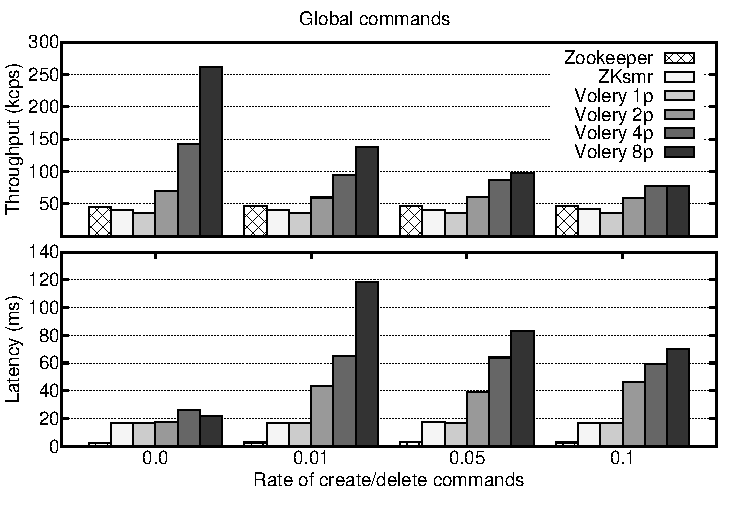
\includegraphics[width=0.9\columnwidth]{{graphs/results/zk_multipartition/plot_tp_lat_multi_global}.pdf}
\end{minipage}
\begin{minipage}[b]{0.5\linewidth}
\centering
      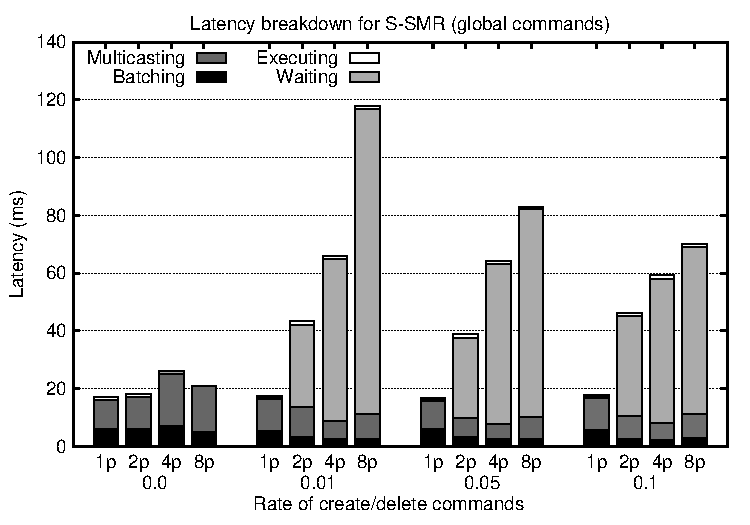
\includegraphics[width=0.9\columnwidth]{{graphs/results/zk_multipartition/timelines_global}.pdf}
\end{minipage}
\caption{Throughput and latency versus rate of create/delete commands (in-memory storage, 1000-bytes commands). Throughput is shown in units of a thousand commands per second (kcps). Latencies shown corresponds to 75\% of the maximum throughput.}
\label{fig:zkglobal}
\end{figure*}

\begin{figure*}

\begin{minipage}[b]{0.3333\linewidth} % A minipage that covers half the page
\centering
      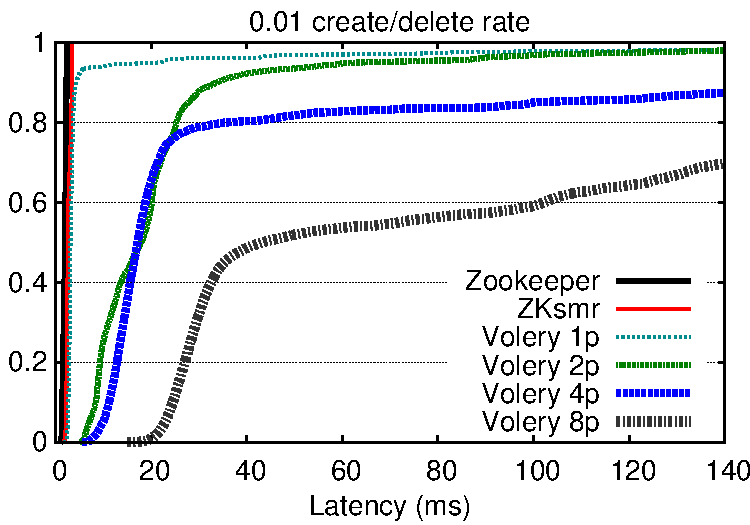
\includegraphics[width=0.9\columnwidth]{{graphs/results/zk_multipartition/plot_latency_cdfs_globalrate_0.01}.pdf}
\end{minipage}
\begin{minipage}[b]{0.3333\linewidth}
\centering
      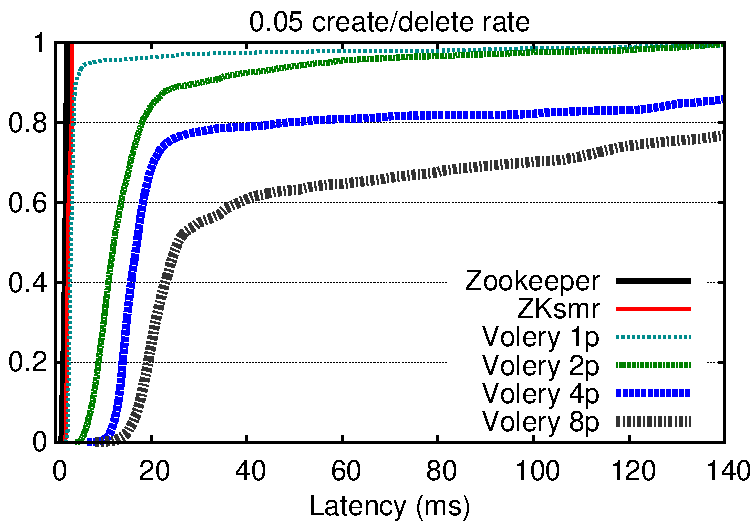
\includegraphics[width=0.9\columnwidth]{{graphs/results/zk_multipartition/plot_latency_cdfs_globalrate_0.05}.pdf}
\end{minipage}
\begin{minipage}[b]{0.3333\linewidth}
\centering
      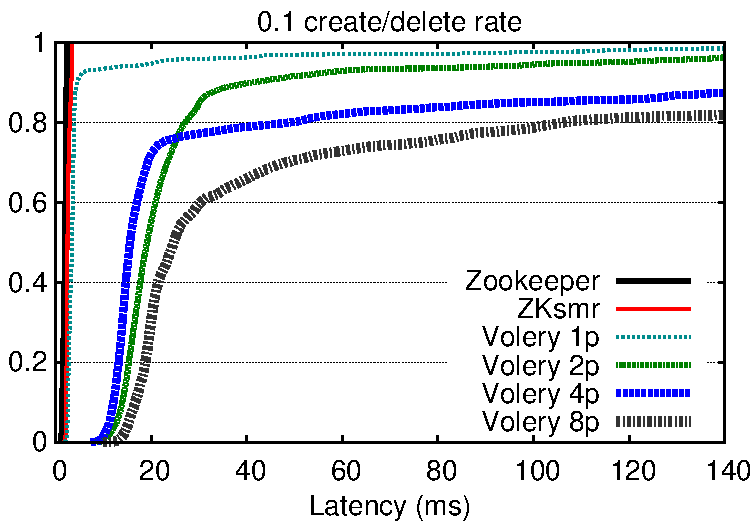
\includegraphics[width=0.9\columnwidth]{{graphs/results/zk_multipartition/plot_latency_cdfs_globalrate_0.1}.pdf}
\end{minipage}
\caption{Cumulative distribution function (CDF) of latency for different rates of create/delete commands (in-memory storage, 1000-bytes commands).}
\label{fig:zkglobalcdf}
\end{figure*}



We can see in Figure \ref{fig:zkglobal} (top left) that Volery scales throughput with the number of partitions for all configurations but the exceptional case of 10\% of global commands when augmenting the number of partitions from 4 to 8.
Moreover, Volery with two partitions outperforms the Zookeeper in all experiments.
The major drawback of Volery under global commands is that to ensure linearizability, partitions must exchange signals: as \verb#create# and \verb#delete# commands are multicast to all partitions, no server can send a reply to a client before receiving a signal from \emph{all} other partitions when executing such a command. 
This explains the significant increase in latency shown in Figure \ref{fig:zkglobal} (bottom left), as global commands are added to the workload: as the number of partitions increases, so does the average latency. 
As we can see in Figure \ref{fig:zkglobal} (right), this extra latency comes from the servers waiting for signals from other partitions.

Figure \ref{fig:zkglobalcdf} shows the latency CDFs for the workloads with global commands. 
For experiments with more than one partition, the rate of messages with high latency is much higher than the rate of global commands. 
This happens due to a ``convoy effect": local commands may be delivered after global commands, having to wait for the latter to finish.
%This happens due to a ``convoy effect": local commands may be delivered after global commands and, therefore, must wait for the latter to finish executing.%, which delays the execution of the local commands.

%\subsection{Chirper experiments}
%
%TODO: every request touching x partitions; 1 experiment for each x in \{1, 2, 4, 8\}, when the system has p partitions, with p in \{1, 2, 4, 8\}
%
%We have also simulated a social network using detailed statistics of real Twitter usage, which can be found online.\footnote{http://www.sysomos.com/insidetwitter/} In such experiment, we simulated 100,000 users. Each user followed $f$ friends, where such friends were divided among $p$ partitions. The resulting graph was made so that each user would have $r$ followers. For each user, we decide values $f$, $p$ and $r$ randomly, based on the statistics we have found: we made both $f$ and $r$ follow a Zipfian distribution with size 100 and skew 1, while $p$ followed a Zipfian distribution with size $P$ (total number of partitions in the system) and skew 1. Also, according to the statistics we have used, 5\% of all Twitter users were responsible for 75\% of all Twitter activity (i.e., number of tweets), while 10\% were responsible for 86\% of all activity, and so on, approximately fitting a Zipfian distribution with size 100 and skew 1.6, where the most active users were the ones with most followers, so our simulated social network also had this characteristic. We used the same distribution for timeline requests, having the users with most friends (i.e., those who follow the most people) requesting their timeline more frequently than other users.

%!TEX root =  main.tex
\section{Related work}
\label{sec:rw}

State machine replication~\cite{Kapritsos:2012um, kotla2004htbft, Lam78, santos2013htsmr, Sch90} provides strong consistency guarantees, which come from total order and deterministic execution of commands.
%Deterministic execution is usually ensured by having every replica execute commands sequentially.
Since consistent ordering is fundamental for SMR, some authors proposed to optimize the ordering and propagation of commands.
% (i.e., the atomic broadcast layer of the system).
For instance, \cite{kapritsos2010scalable} proposes to divide the ordering of commands between different clusters: each cluster orders only some requests, and then forwards the partial order to every server replica, which then merges the partial orders deterministically into a single total order that is consistent across the system.
In~\cite{biely2012spaxos}, Paxos~\cite{Lamport:1998ea} is used to order commands, but it is implemented in a way that avoids overloading the leader process, which would turn it into a bottleneck.

Multi-threaded execution is a potential source of non-determinism, depending on how threads are scheduled to be executed in the operating system.
Some works attempted to circumvent this problems and come up with a multi-threaded, yet deterministic implementation of SMR.
In \cite{santos2013htsmr}, the authors propose to parallelize the receipt and dispatching of commands, while executing commands sequentially.
In \cite{kotla2004htbft}, application semantics is used to determine which commands can be executed concurrently and still produce a deterministic outcome (e.g., read-only commands).
In \cite{Kapritsos:2012um}, commands are tentatively executed in parallel.
After the parallel execution, replicas verify whether they reached a consistent state; if not, commands are rolled back and re-executed sequentially.

Many database replication schemes aim at achieving high throughput by relaxing consistency, that is, they do not ensure linearizability.
In deferred-update replication \cite{chundi96dur, kobus2013hybrid, sciascia2012sdur, SousaOMP01}, replicas commit read-only transactions immediately, not always synchronizing with each other.
Although this indeed improves performance, it allows non-linearizable executions.
Database systems usually ensure serializability \cite{BHG87} or snapshot isolation \cite{LinKJPA09}, which do not take into account real-time precedence of different commands among different clients. 
For some applications, these consistency levels may be enough, allowing the system to scale better, but services that require linearizability cannot be implemented with such techniques.

Efforts to make linearizable systems scalable have been made in the past~\cite{bezerra2014ssmr, corbett2013spanner, Glendenning2011, hoang2016, Marandi11}.
In \cite{Glendenning2011}, the authors propose a scalable key-value store based on DHTs, ensuring linearizability, but only for requests that access the same key. 
In \cite{Marandi11}, variant of SMR is proposed in which data items are partitioned but commands have to be totally ordered.
Spanner~\cite{corbett2013spanner} uses a separate Paxos group per partition and, to ensure strong consistency across partitions, clocks are assumed to be synchronized.
Although the authors say that Spanner works well with GPS and atomic clocks, if clocks become out of synch beyond tolerated bounds, correctness is not guaranteed.
\ssmr{}~\cite{bezerra2014ssmr} ensures consistency across partitions without any assumption about clock synchronization, but relies on a static partitioning of the state.
\dssmr{}~\cite{hoang2016} extends \ssmr\ by allowing state variables to migrate across partitions in order to reduce multi-partition commands.
However, \dssmr{} implements repartitioning in a very simple way that does not perform very well in scenarios with weak locality.
\dynastar\ improves on \dssmr\ by employing well-known graph partitioning techniques to decide where each variable should be.
Moreover, \dynastar\ dillutes the cost of repartitioning by moving variables on-demand, that is, only when they are accessed by some command.

Graph partitioning is an interesting problem with many proposed solutions~\cite{Abou-Rjeili:2006,kernighan1970efficient,hendrickson2000graph}.
In this work, we do not introduce a new graph partitioning solution, but instead we use a well-known one (METIS~\cite{Abou-Rjeili:2006}) to partition the state of a service implemented with state machine replication.
Similarly to \dynastar{}, Schism~\cite{curino2010sch} and Clay~\cite{SerafiniTEPAS16} also use graph-based partitioning to decide where to place data items in a transactional database.
In either case, not much detail is given about how to handle repartitioning dynamically without violating consistency.
Sword~\cite{quamar2013sword} is another graph-based dynamic repartitioning technique.
It uses a hypergraph partitioning algorithm to distribute rows of tables in a relational database across database shards.
Sword does not ensure linearizability and it is not clear how it implements repartitions without violating consistency.
E-Store~\cite{taft2014est} is yet another repartitioning proposal for transactional databases.
It repartitions data according to access patterns from the workload.
It strives to minimize the number of multi-partition accesses and is able to redistribute data items among partitions during execution.
E-Store assumes that all non-replicated tables form a tree-schema based on foreign key relationships.
This has the drawback of ruling out graph-structured schemas and \mbox{$m$-$n$} relationships.
\dynastar\ is a more general approach that works with any kind of relationship between data items, while also ensuring linearizability.

Some replication schemes are ``dynamic'' in that they allow the membership to be reconfigured during execution (e.g., \cite{birman2010dsr,dustdar2007soc,guessoum2003dar}).
For instance, a multicast layer based on Paxos can be reconfigured by adding or removing acceptors. 
These systems are dynamic in a way that is orthogonal to what \dynastar\ proposes.
%\dynastar\ consists of allowing the \emph{state partitioning}, that is, which state variables belong to which partition, to change dynamically.
%The greatest challenge that is addressed by \dynastar\ is how to provide such a solution, with a dynamic partitioning oracle, while ensuring a very strong level of consistency (linearizability), as variables are created, deleted, and moved across partitions, based on the access patterns of the workload.



\section{Conclusion}
\label{sec:conclusion}

This work introduces S-SMR, a scalable variant of the well-known state-machine replication technique. 
S-SMR differs from previous related works in that it allows throughput to scale with the number of partitions without weakening consistency. 
To evaluate S-SMR, we developed the Eyrie library and implemented Volery, a Zookeeper clone, with Eyrie.
Our experiments demonstrate that in deployments with 8 partitions (the largest configuration we can deploy in our infrastructure) and under certain workloads, throughput experienced an 8-time improvement, resulting in ideal scalability.
Moreover, Volery's throughput proved to be significantly higher than Zookeeper's.

\section*{Acknowledgements}
\label{sec:acknowledgements}

This work was supported in part by the Swiss National Science Foundation under grant number 146404. Robbert van Renesse is supported in part by grants from AFOSR, NSF, DARPA, ARPA-e, MDCN/iAd, Microsoft Corporation, Facebook Inc., and Amazon.com.% We also thank Samuel Benz and Leandro Pacheco de Sousa for the discussions.

%\section*{Acknowledgment}
%Thank the reviewrs

%\bibliographystyle{IEEEtran}
\bibliographystyle{ieeetr}
%\bibliographystyle{abbrvnat}
\bibliography{references_short}
%\bibliography{references}



\end{document}